% main.tex, to be used with thesis.tex
% This contains the main work of your thesis.

%\bibliography{thesis}  % uses the references stored in Chapter1Radar.bib

\chapter{Data Persistence for Sensor Networks: A Case Study for NetBEAMS}
\label{chap:netbeams-overview}

This chapter presents the main motivation and scope of of this dissertation.
The infrastructure of SF-BEAMS is presented as a real-world environmental
sensor network, deployed by the department of Biology at the San Francisco State
University. It serves as the foundation of the execution of NetBEAMS, a
joint project between the department of Biology and the Computer Science.
As an alternative approach for data collection, NetBEAMS is used to
automate the data management and collection process of SF-BEAMS. However, it
offered different open problems, including Data Persistence. Therefore, the
scope of the solution presented in the following sections and chapters are
based in the case study presented in this current chapter.

\section{SF-BEAMS: a Marine Sensor Network for Water Quality Monitoring}

The San Francisco Bay Environmental Assessment and Monitoring Station, or
SF-BEAMS \cite{sfbeams2006}, is a marine sensor network operated by the Romberg
Tiburon Center (RTC), whose main focus is the study of complex marine and
estuarine environments using the SF-BEAMS sensors. The network is deployed
offshore of its pier located on the banks of the San Francisco Bay at the
Tiburon Island, California, being operated by the department of Biology from
San Francisco State University.

\subsection{The SF-BEAMS Infrastructure}

The SF-BEAMS sensor network is responsible for providing data for water quality
monitoring, as well as weather and surface conditions. Figure
\ref{fig:sf-beams} shows a picture taken from the SF-BEAMS web-cam placed
in-site.

\begin{figure}[!b]
  \centering
    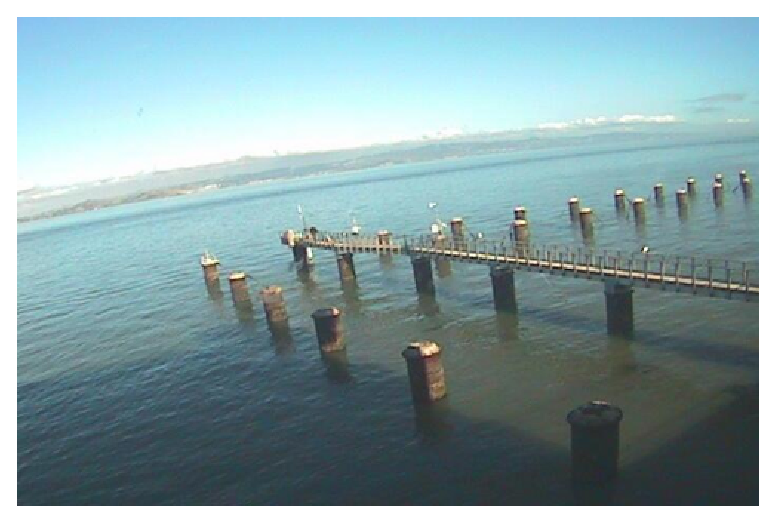
\includegraphics[scale=0.7]{../diagrams/cam_image-oct15}
  \caption{Picture of the SF-BEAMS Network, at the RTC pier. Tiburon, CA.}
  \label{fig:sf-beams}
\end{figure}

In general, the SF-BEAMS network infrastructure contains heterogeneous wired and
wireless devices standing on pilons docked in the pier, where each of them is
responsible for observing different conditions of the area, as well as having
its own mechanisms for internal storage for the collected data. In this way,
data can be directly transferred to the labs via ethernet cables or collected
manually by a laptop computer.

\subsection{SF-BEAMS produced data and collection process}
\label{sec:sfbeams}

As described in section \ref{sec:sn-infrastructure}, sensor devices generate
its observed data based on properties of measurements defined by its
manufacturer. SF-BEAMS can be seen a single-hop star sensor network containing
different instances of sensors, including the "YSI 6600 ESD V2", as seen on
figure \ref{fig:ysi-device}, which is a powerful water quality monitoring
device that produces around 52 bytes (13x4 Bytes) on a single real-time data
stream as shown on table \ref{tab:ysi-data-stream}.

\begin{figure}[!b]
  \centering
  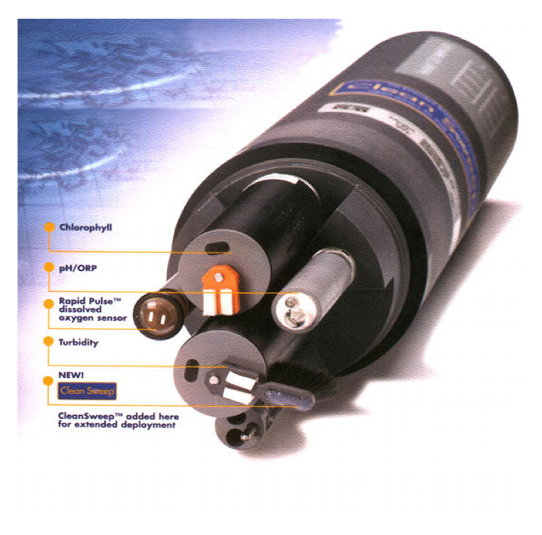
\includegraphics[scale=0.7]{../diagrams/ysi-device}
  \caption{Picture of the case study sonde device: YSI 6600 ESD V2}
  \label{fig:ysi-device}
\end{figure}

\begin{table}
    \caption{YSI Data Stream}
    \begin{center}
        \begin{tabular}{lr}
  12.20    192    179 5588.40   0.09   0.084   0.059  7.98   -79.6   99.5  8.83 
  0.4     8.7
        \end{tabular}
    \end{center}
    \label{tab:ysi-data-stream}
\end{table}

In order to have access to the observed data, the network staff downloads
the data using one of the device's connection such as the RS-232 serial
connector \cite{rs232}. Then, the data is transferred to the RTC labs for
archival, where it is described, indexed and distributed to its main users.
According to one of its staff members, the infrastructure of the SF-BEAMS in
May 2009 was comprised of the following:

\begin{itemize}
  \item Among other devices, 5 YSI sondes in operation at the RTC pier;
  \item Each YSI sonde produces 52 Bytes for each its observations;
  \item The sampling frequency rate could be configured in ranges of 1, 6 or
  15 minutes, depending on the specification;
  \item Data for final users are published with Provenance Data regarding time,
  but no metadata regarding the origin of data.
\end{itemize}

Considering the infrastructure previously described, the size of the data
produced by the YSI sonde sensors at the RTC pier can estimated by its
measurement frequency as follows:

\begin{table}
    \label{tab:ysi-data-distribution}
    \caption{Amount of data produced by the RTC's YSI sondes}
        \begin{center}
        \begin{tabular}{|c|c|c|c|c|c|c|}\hline 
        \textbf{YSIs} & \textbf{Rate} & \textbf{Hourly} & \textbf{Daily} &
        \textbf{Weeky} & \textbf{Monthly} & \textbf{Yearly}\\\hline 
        1 & 1 min & 3.04 Kb & 73.12 Kb & 511.87 Kb & 1.99 Mb & 23.99 Mb\\\hline 
        5 & 6 min & 15.23 Kb & 365.62 Kb & 2.5 Mb & 9.99 Mb & 119.97 Mb\\\hline 
        1 & 15 min & 0.5 Kb & 12.18 Kb & 85.31 Kb & 341.25 Kb & 3.99 Mb\\\hline 
        5 & 1 min & 2.54 Kb & 60.93 Kb & 426.56 Kb & 1.67 Mb & 19.99 Mb\\\hline
        1 & 6 min & 0.2 Kb & 4.87 Kb & 34.12 Kb & 136.5 Kb & 1.6 Mb\\\hline 
        5 & 15 min & 1.0 Kb & 24.37 Kb & 170.62 Kb & 682.5 Kb & 7.99 Mb\\\hline
        \end{tabular}
        \end{center}
\end{table}

As it is shown, the data produced by this type of sensor runs in the order of
at most hundreds of Megabytes a year for a maximun of \textbf{483,840} samples,
what can be considered a very low data storage requirement as compared to
other networks. Upon collecting the data from sensors, the RTC lab staff use
automation scripts written in Matlab to process, index and distribute the raw
data in different formats, including the OPeNDAP \cite{opendap}, a format
widely used in the research institutions that promotes easier data exchange
among them. The access to the archived data is done by using the OPeNDAP
server is located at http://sfbeams.sfsu.edu:8080/opendap, as a request and
the related output for one of the YSI devices can be see in Listing
\ref{file:rtc-ysi-opendap}.

\subsection{Taxonomic Classification of SF-BEAMS}

In order to distinct each of the properties of the SF-BEAMS sensor
networks, consider the following list as a classification of the data
persistence mechanisms from the sensor network used by the project:

\begin{itemize}
  \item \textbf{The Purpose of Sensor Data}: the data from SF-BEAMS is purely
  used for \textbf{Data Archival} purposes, since they are stored in the RTC's
  lab as part of the collaboration research project that monitors each part of
  the California's coast. The data sets are distributed by specific date in a
  yearly calendar;
  \item \textbf{The Location of the Sensor Data}: it is clear that the purpose
  of data is directly related to its location and, as consequence, the strategy
  of \textbf{External Data Storage} is used to store its collected data at the
  network sink at the RTC's labs;
  \item \textbf{Data Model}: no data model is used by the RTC's staff to model
  the data. A simple transformation of the data collected from the sensors
  directly to spreadsheets, using comma-delimited values, is used. That is, the
  data mode used is \textbf{Schema-less};
  \item \textbf{Data Provenance}: data is stored in files with conventions that
  takes the time when the data was collected. The contents of the files include
  the \textbf{Data Identity} and \textbf{Time Dimensions}, as shown in
  the samples collected and shown in Listing \ref{file:rtc-ysi-opendap};
  \item \textbf{Query Processing Mechanism}: data is queried in a
  \textbf{Centralized} fashion, due to the nature of its purpose and locality;
  \item \textbf{Database System Organization}: there are no database in place.
  The SF-BEAMS labs use the OPeNDAP Hyrax server as a middleware used to read
  and interpret the collected data. 
\end{itemize}

\section{NetBEAMS: a component-based approach for SF-BEAMS}
\label{sec:problem-requirements}

Although the execution of the RTC's sensor network can be operated as it
described in the previous sections, \cite{netbeams2009} described some
operational challenges faced by the RTC staff during regular activities during
the data collection process. It was clear to the research group that SF-BEAMS
could have not only its data gathering process automated, but also its data
management and distribution. By the use of COTS\footnote{Common-Off-The-Shelf
designates a product that is produced and sold in bulk} embedded
devices and open-source \cite{open-source} software, the research group 
developed a second version of NetBEAMS, a component-based approach suggested
to improve the operational activities from SF-BEAMS by using systems
automation techniques. In brief, one of the open problems of NetBEAMS was
regarding Data Persistence, the main motivation of this dissertation.

The Networked Bay Environmental Assessment and Monitoring System, or NetBEAMS, 
is a work-in-progress joint project proposed by the department of Computer
Science and the RTC at San Francisco State University. The main reason for the
inception of NetBEAMS is the potential to decrease operational costs and speed
the data gathering process. In the current state of SF-BEAMS, Biologists need
to manually collect the data from the sensor devices in order to take them to
the network sink (lab) for further processing. For this reason, the Data
Sensor Platform (DSP) \cite{netbeams2009} was proposed as the system
architecture that can address the operation of SF-BEAMS. Therefore, an in-depth
detail of the the DSP Platform, its architecture and data gathering process
can are provided in the appendix section \ref{sec:dsp-details}, and may be
referred at any time.

The scope of this work then is defined as to provide a persistence layer for
NetBEAMS, making a selection of a persistence layer that is complaint to the
taxonomical classification of SF-BEAMS. Furthermore, the technology to be
selected for the persistence layer must take into account the requirements of
NetBEAMS primary users such as Computer Science researchers, as well as end
users such as Biologists from the RTC laboratories.

\subsection{Requirements for NetBEAMS Data Use}

The main reason for the operation of SF-BEAMS using NetBEAMS's automated
approach is that it can potentially reduce operational costs and improve the
data collection process. In review of this, the scope of a persistence layer
can be summarized as a group of functional and non-functional requirements in
order to select a database system for the sensor network supported by NetBEAMS.

\subsection{Functional Requirements}

\begin{itemize}
  \item Reuse the NetBEAMS infrastructure and develop a component responsible
  for data persistence in a database system;
  \item The Persistence System must obey to the characteristics of the
  categorization of SF-BEAMS used by the taxonomies. 
\end{itemize}

\subsection{Non-Functional Requirements}

\begin{itemize}
  \item The data model used to describe the data must not impose restrictions
  to the users of the system: Biologists and students without expertise in
  Database Systems;
  \item Data Representation must be similar to the ones used by RTC,
  with a more human-readable format;
  \item Scalable System with low degree of maintanance, in a way that data
  gathering service should be able to manage the system with less service
  interruption;
  \item Data must be searchable in near-real-time with good performance, as
  compared to the time when data was collected to the time when they are available;
  \item Easy data integration and export capabilities must be also taken into
  account;
  \item The database system must be free of charge, following the
  implementation specifications of NetBEAMS.
\end{itemize}